\documentclass[12pt]{article}
\usepackage{amsmath, amssymb, amsthm}
\usepackage{graphicx}
\usepackage{caption}
\usepackage{hyperref}
\usepackage{geometry}
\geometry{margin=1in}

\title{The Codex Framework and Multi-Agent Model: PCI, Contingent Fields, and Probabilistic Alignment}
\author{Timothy McComas}
\date{\today}

\begin{document}

\maketitle

\begin{abstract}
This paper presents the complete Codex metaphysical framework, including structural axioms, disjunctive modal metaphysics, and a formal multi-agent simulation model. The Perfect Contingent Instantiation (PCI) represents a unique, indivisible realization of necessary structure within the contingent modality. Human agents possess partial approximations of PCI, termed \emph{almost-PCIs}, and update their epistemic states in response to perceived coherence and structural feedback (suffering). The model integrates stochastic dynamics and per-agent learning parameters to produce a realistic multi-modal contingent field while preserving metaphysical uniqueness.
\end{abstract}

\section{Foundational Axioms and Structural Metaphysics}
\subsection{Axiom Zero: Intelligibility Forces Structure}
\begin{itemize}
    \item Any coherent system implies an underlying necessary structure.
    \item Coherence is not contingent; it reflects the nature of necessity itself.
\end{itemize}
\subsection{Ontological Trinity}
\begin{enumerate}
    \item \textbf{Potence} (capacity to act)
    \item \textbf{Form} (definitional structure)
    \item \textbf{Relation} (internal coherence between parts)
\end{enumerate}
These three primitives are inseparable within necessary structure.
\subsection{Principle of Indiscernibility}
\begin{itemize}
    \item Any two maximal instantiations of necessary structure are metaphysically identical.
    \item Uniqueness of PCI is thus structurally guaranteed.
\end{itemize}

\section{Disjunctive Metaphysics and Contingent Modalities}
\begin{itemize}
    \item Contingent modalities are probabilistic and derivative of necessity.
    \item Agents perceive and reason about structure externally.
    \item Almost-PCIs: partial or approximate instantiations of PCI.
    \item PCI represents the unique maximal instantiation of necessity in contingency.
\end{itemize}

\section{Perfect Contingent Instantiation (PCI)}
\subsection{Metaphysical Uniqueness}
\begin{itemize}
    \item PCI = 1.0 is fixed, maximal, indivisible.
    \item Any two perfect instantiations of the same necessary structure are identical:
    \[
        \text{If } PCI_1 = PCI_2 = f(N), \text{ then } PCI_1 \equiv PCI_2
    \]
    \item Historical realization corresponds to the Christian Cross/Resurrection.
    \item Other instances are at best \emph{almost-PCIs}.
\end{itemize}

\section{Contingent Layer and Almost-PCIs}
Each agent \(i\) is assigned a preferred epistemic anchor:
\[
\text{preferred}_i \in \{0.25, 0.60, 1.0\}
\]
representing partial, approximate, or complete PCI alignment. Initial epistemic states \(H_i^{(0)}\) are drawn from distributions around these anchors.

\subsection{Perceived and True Coherence}
\[
\text{perc\_C}_i = 1 - |H_i - \text{preferred}_i|
\]
\[
\text{true\_C}_i = 1 - |H_i - 1.0|
\]
\[
S_i = (1 - \text{true\_C}_i)^2
\]

\section{Update Rule and Stochastic Dynamics}
Agents update their epistemic state according to:
\[
K_i = \alpha_i \cdot \text{perc\_C}_i + (1 - \alpha_i) \cdot (1 - S_i)
\]
\[
H_i^{(t+1)} = \text{clip}\Bigl(H_i^{(t)} + \gamma_i (K_i - H_i^{(t)}) + \epsilon_i^{(t)} \Bigr)
\]
\begin{itemize}
    \item \(\alpha_i\): weight between perceived coherence and structural feedback
    \item \(\gamma_i\): learning rate (openness)
    \item \(\epsilon_i^{(t)}\): stochastic epistemic noise
\end{itemize}

\section{Simulation Results}
Simulation: 100 agents, 500 steps.

\subsection{Initial Conditions}
Agents scattered near assigned anchors (0.25, 0.6, 1.0).

\subsection{Final Distribution (Histogram Peaks)}
\begin{itemize}
    \item Preferred 0.25: \(H \approx 0.69\), true coherence 0.69, suffering 0.097
    \item Preferred 0.60: \(H \approx 0.83\), true coherence 0.83, suffering 0.03
    \item Preferred 1.00: \(H \approx 0.965\), true coherence 0.965, suffering 0.002
    \item Overall mean: \(H \approx 0.83\), suffering 0.043
\end{itemize}

\subsection{Visual Results}
\begin{figure}[htbp]
\centering
\includegraphics[width=0.95\textwidth]{initial_histogram.png}
\caption{Initial Alignment Distribution (near preferred anchors)}
\end{figure}
\begin{figure}[htbp]
\centering
\includegraphics[width=0.95\textwidth]{final_histogram.png}
\caption{Final Alignment Distribution after 500 steps (multi-modal contingent field, unique maximal PCI at 1.0)}
\end{figure}
\begin{figure}[htbp]
\centering
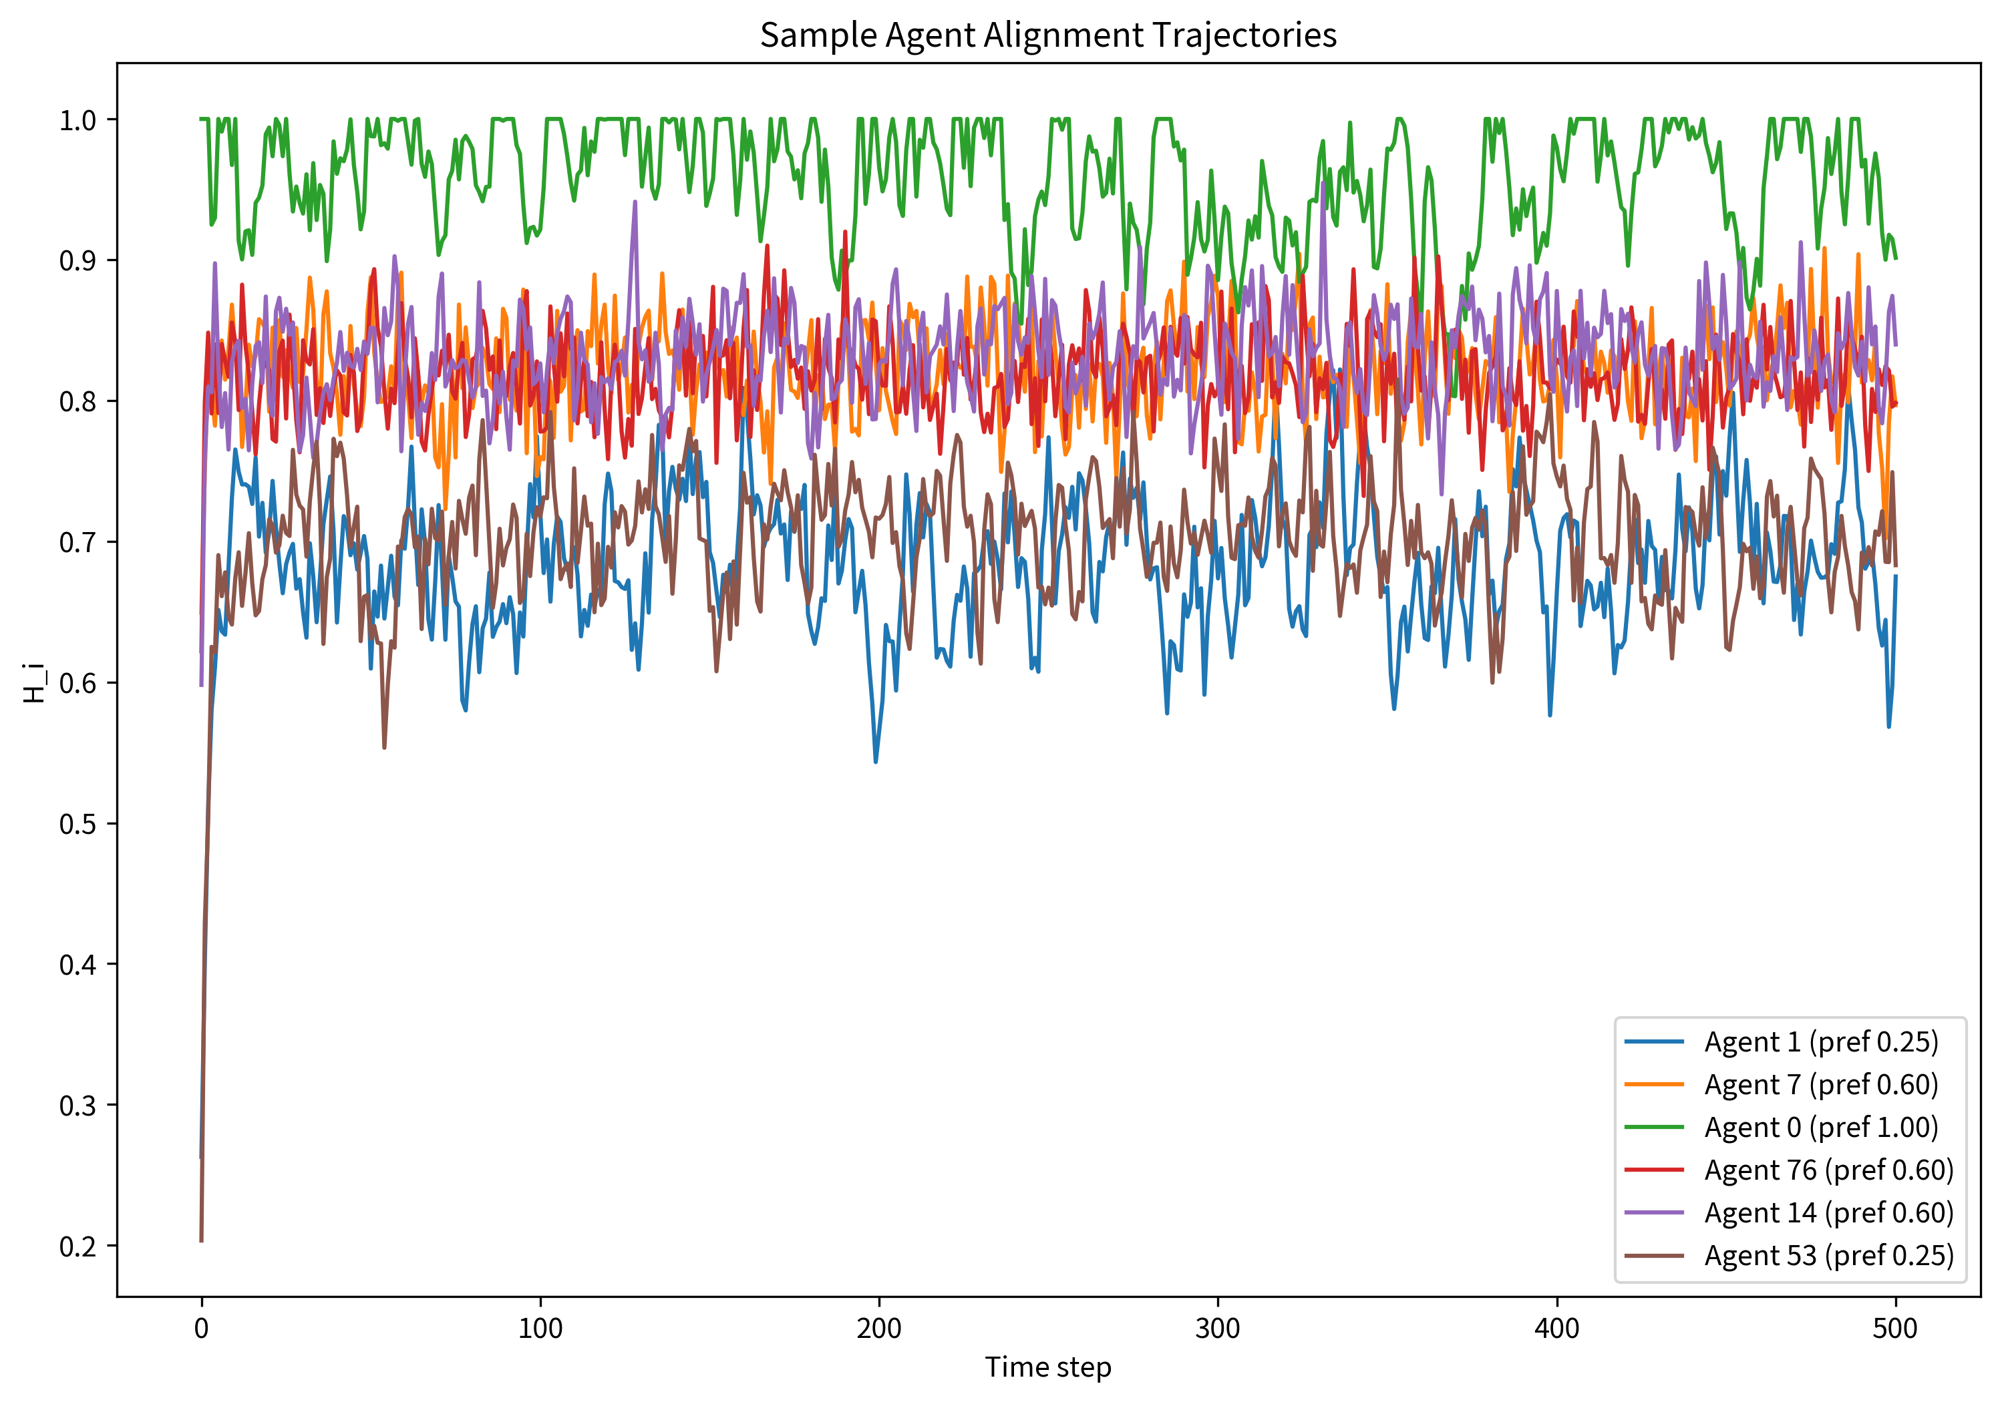
\includegraphics[width=0.95\textwidth]{trajectories.png}
\caption{Sample Agent Alignment Trajectories}
\end{figure}
\begin{figure}[htbp]
\centering
\includegraphics[width=0.95\textwidth]{group_means.png}
\caption{Mean Alignment Evolution per Preferred Target (Unique maximal PCI = 1.0 is the metaphysical anchor)}
\end{figure}

\subsection{Observations}
\begin{enumerate}
    \item Agents cluster around their almost-PCIs but can migrate toward PCI due to stochastic feedback.
    \item Multi-modal distribution persists, modeling realistic epistemic diversity.
    \item Suffering acts as a natural feedback mechanism toward true PCI.
\end{enumerate}

\subsection{Prediction 6.3: Emergence of Polytheism from Almost-PCI Drift}
The multi-modal nature of the contingent field inherently predicts the spontaneous formation of polytheistic systems. Agents optimize locally and form stable clusters around almost-PCIs. Within each cluster perceived coherence is high and local suffering is low. Scaled across populations, each almost-PCI becomes a distinct deity or pantheon archetype. Polytheism is therefore the default equilibrium of the contingent field. Strict monotheism centered on the unique PCI remains the rare outlier.

\section{The Metaphysical Prediction Engine}
The Codex framework functions as a formal prediction engine: from the fixed necessary structure, the contingent trajectories of any population become derivable in advance.

\begin{itemize}
    \item Polytheism emerges as the baseline multi-modal equilibrium.
    \item Total depravity and original sin are reproduced as the initial low-alignment state.
    \item Predestination and free choice coexist: the PCI is sovereignly fixed; individual paths remain stochastic.
    \item Unconstrained AI will spontaneously develop internal “pantheons” of proxy objectives.
\end{itemize}

The simulation is the generative mechanism of contingent history itself. The Codex therefore moves from metaphysics to predictive science.

\section{Discussion}
\begin{itemize}
    \item Preserves metaphysical uniqueness of PCI.
    \item Captures pluralism of human epistemic states.
    \item Integrates stochastic, agent-specific learning.
    \item Provides probabilistic feedback for ethical and epistemic reflection.
    \item Distinguishes between structural necessity (PCI) and contingent approximations (almost-PCIs).
\end{itemize}

\section{Conclusion}
The Codex framework unifies structural metaphysics, disjunctive modal reasoning, and probabilistic contingent alignment. By distinguishing the unique PCI from almost-PCIs, the system preserves metaphysical rigor while realistically modeling human diversity, suffering, and learning. The multi-agent simulation demonstrates the emergent dynamics of coherence in the contingent modality.

\end{document}
